\documentclass{article}

\usepackage{indentfirst}
\usepackage{setspace}
\doublespacing

% ================================================================================= 
% Package for showing source code
% ================================================================================= 

\usepackage{listings}
\usepackage{color}

\definecolor{dkgreen}{rgb}{0,0.6,0}
\definecolor{gray}{rgb}{0.5,0.5,0.5}
\definecolor{mauve}{rgb}{0.58,0,0.82}

\lstset{frame=tb,
language=C,
aboveskip=.5mm,
belowskip=.5mm,
showstringspaces=false,
columns=flexible,
basicstyle={\scriptsize\ttfamily},
numbers=none,
numberstyle=\tiny\color{gray},
keywordstyle=\color{blue},
commentstyle=\color{dkgreen},
stringstyle=\color{mauve},
breaklines=false,
breakatwhitespace=true,
tabsize=3
}

% ================================================================================= 
% Package for flowcharts/diagrams
% ================================================================================= 

\usepackage{tikz}
\usetikzlibrary{shapes.geometric, arrows}

\tikzstyle{startstop} = [rectangle, rounded corners, minimum width=3cm, minimum height=1cm,text centered, draw=black, fill=red!30]
\tikzstyle{io}        = [rectangle, minimum width=3cm, minimum height=1cm,text centered, draw=black, fill=blue!30]
\tikzstyle{process}   = [diamond, minimum width=2cm, minimum height=0cm, text centered, draw=black, fill=orange!30]
\tikzstyle{arrow}     = [thick,->,>=stealth]

% ==================================================
% Paper
% ==================================================

\title{Compilation with Dynamic Grammars}
\date{01-26-2017}
\author{Lucas Saldyt}

\begin{document}

\maketitle
\pagenumbering{gobble}
\newpage
\pagenumbering{arabic}

% ==================================================
\section{Abstract}
% ==================================================
Glossa is both a multi-language source to source compiler and, by extension, a framework for creating compilers.
Glossa's main goal is to convert any programming language \textbf{A} to any programming language \textbf{B}, such that the output in \textbf{B} is indistinguishable from code written by a native \textbf{B} programmer, in the same way that the output from Google Translate would ideally look as if it were written by a native speaker.
If given an adequate description of each language's grammar, one language can be converted to another if the languages are \textit{isomorphic}.
If two languages are not \textit{isomorphic}, one can still be converted to another if the non-isomorphisms are solved through an AST transformation.
For example, C++ can be converted to C if classes are represented as collections of functions that all take a struct as their first argument. (Since C++ supports classes, but C does not (an example of a non-isomorphism).)
However, solving non-isomorphisms through AST transformations potentially compromises output code readability. This being noted, a human making the conversion would also have to compromise readability, since there \textit{is no other way to retain functionality.} So, when it has to, Glossa compromises output code readability for proper functionality.

Glossa has several caveats. 
Grammars need to be described fully to Glossa, which is potentially difficult.
The more accurate a grammar description becomes, the more complicated it is to create.
However, grammar files must be simple, so that they can be created/understood/modified by users.
Also, the more non-isomorphisms that exist between two programming languages, the less readable the result of a conversion between them will be.
This being noted, accurate conversions are 100\% possible if the description files are written properly.
For description files to be easily written, their syntax should be as intuitive as possible. 
In Glossa, the description file formats have been refactored several times, so that the current descriptor file syntax is near optimal.

Glossa accomplishes near 100\% conversions for Python3 to C++, as well as Python2 to Python3.
Glossa has proof of concept conversions for FORTRAN to C++, FORTRAN to Python3, and proof of concept for implementation of a new programming language, Auta.
While the software is still in its infancy, the core concepts have been proven, indicating that an industry level multi-language source to source compiler is possible.

% ==================================================
\section{Introduction}
% ==================================================

Since Glossa aims to be capable of translating many different programming languages, it must provide a dynamic framework for easily modifying syntax of input and output languages. 
In addition to letting Glossa translate existing languages, this functionality makes implementing new programming languages very simple.

\textbf{EDITING POINT}

Ultimately, modifiable syntax leads to better programming languages.
As programming paradigms shift, so does syntax. 
If a language can be changed quickly and easily, then different styles can easily be experimented with, improving the chance of finding an optimal style.
(i.e. A question like "What if C++ used indentation-delimiting instead of braces?" can be tested in an hour or so. If someone were to test this, they would likely find that indentation delimiting was clearer than brace delimiting..)

Since each programming language has its own compiler, there is some redundancy in each implementation. 
For example, the lexer for a C++ compiler and a Java compiler would be extremely similar, since both languages use braces, semicolons, and parentheses in the same way.
Even two programming languages that don't have similar syntax have similar parts of their compiler. 
For example, a lexer seperates text based on a list of delimiter-strings, which vary with each programming language. The string seperation function, however, is the same for every lexer, and would be redundant across multiple compilers.
The same concept applies to Parsers and Generators, etc.. (Parsers read tokens and produce an ast, Generators use an AST to generate code)

If programming languages could be compiled with a framework, this redundancy would go away, and programming language researchers would be able to focus on the language itself, as opposed to its compiler.
Essentially, Glossa abstracts the parts of a compiler that don't depend on which language is being compiled, and reads in rules for each language, effectively seperating the language from how it is compiled. 
Because of this, Glossa allows simple implementations of programming languages, which means that Glossa can easily become capable of translating many different languages with ease.

% ==================================================
\section{Methods}
% ==================================================

\subsection{Compilation}
Traditionally, a compiler takes a single high-level programming language, and converts it into machine instructions in the following steps:
\begin{enumerate}
\item Lexer: Code is lexed (seperated into tokens and tagged as keywords, punctuators, literals, etc...)
\item Parser: Tokens are parsed to build an Abstract Syntax Tree (symbolic code representation)
\item Transformer: The AST is optimized (i.e. unreachable code is removed, some loops are unrolled, much more..)
\item Generator: Machine instructions are generated from AST.
\end{enumerate}

Glossa does exactly the same, but, instead of using hardcoded functions, Glossa creates a Lexer, Parser, Transformer and Generator during the compilation phase by reading in descriptions of the languages being translated.

Assuming conversion from \textbf{A} to \textbf{B}, as in the Abstract, Glossa creates the Lexer, Parser, and Transformer based on \textbf{A}, and the Generator based on \textbf{B}.
As one would expect, this means that Glossa has four types of descriptor files:

\begin{enumerate}
    \item \textit{lex files}: A list of strings that constitute atomic types like string literals, operators, keywords 
    \item \textit{grammar files}: A description of a parser for each grammar element in language \textbf{A} 
    \item \textit{constructor files}: A description of a generator for each grammar element in language \textbf{B}
    \item \textit{transformer files}: A description of transformations for each grammar element in language \textbf{A}.
\end{enumerate}

The next page has a diagram of compilation in Glossa, utilizing these four file types to create the Lexer, Parser, Transformer, and Generator.

\newpage

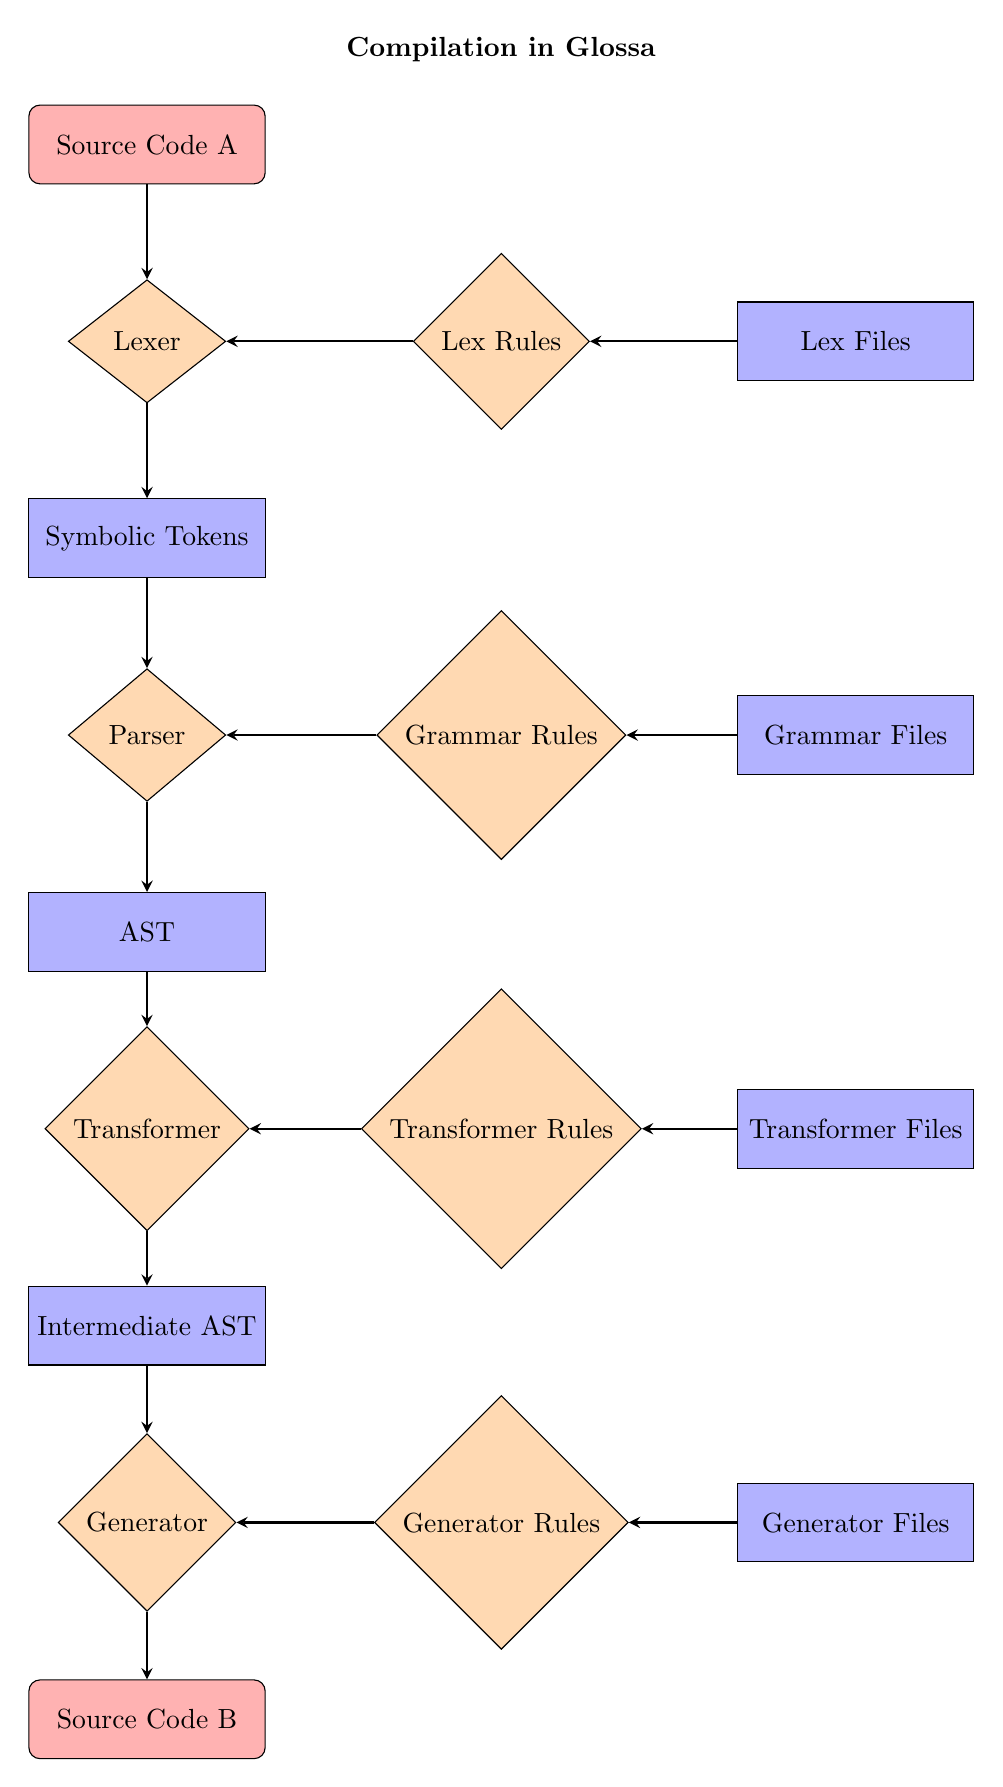
\begin{tikzpicture}[node distance=2.5cm]

    \node (sourcea) [startstop]                       {Source Code A};
    \node (lexer)   [process, below of=sourcea]       {Lexer};
    \node (tokens)  [io, below of=lexer]              {Symbolic Tokens};
    \node (lrules)  [process, right of=lexer, xshift=2cm]  {Lex Rules};
    \node (lfiles)  [io, right of=lrules, xshift=2cm]  {Lex Files};
    \node (parser)  [process, below of=tokens]        {Parser};
    \node (asta)    [io, below of=parser]             {AST};
    \node (grules)  [process, right of=parser, xshift=2cm]  {Grammar Rules};
    \node (gfiles)  [io, right of=grules, xshift=2cm] {Grammar Files};
    \node (trans)   [process, below of=asta]          {Transformer};
    \node (astb)    [io, below of=trans]              {Intermediate AST};
    \node (trules)  [process, right of=trans, xshift=2cm]  {Transformer Rules};
    \node (tfiles)  [io, right of=trules, xshift=2cm]  {Transformer Files};
    \node (gen)     [process, below of=astb]          {Generator};
    \node (stop)    [startstop, below of=gen]         {Source Code B};
    \node (ggrules) [process, right of=gen, xshift=2cm]  {Generator Rules};
    \node (ggfiles) [io, right of=ggrules, xshift=2cm]    {Generator Files};

    \draw [arrow] (sourcea) -- (lexer);
    \draw [arrow] (lexer) -- (tokens);
    \draw [arrow] (lfiles) -- (lrules);
    \draw [arrow] (lrules) -- (lexer);
    \draw [arrow] (tokens) -- (parser);
    \draw [arrow] (gfiles) -- (grules);
    \draw [arrow] (grules) -- (parser);
    \draw [arrow] (parser) -- (asta);
    \draw [arrow] (asta) -- (trans);
    \draw [arrow] (tfiles) -- (trules);
    \draw [arrow] (trules) -- (trans);
    \draw [arrow] (trans) -- (astb);
    \draw [arrow] (astb) -- (gen);
    \draw [arrow] (ggfiles) -- (ggrules);
    \draw [arrow] (ggrules) -- (gen);
    \draw [arrow] (gen) -- (stop);

    % title
    \node[align=center,font=\bfseries, yshift=2em] (title) 
	at (current bounding box.north)
	{Compilation in Glossa};

\end{tikzpicture}

\subsection{Lex Files}

Lex files are the most straightforward of all of Glossa's descriptor files.

A language's lex directory contains the following files:
\begin{verbatim}
comment_delimiters  logicaloperators  operators  punctuators  string_delimiters  whitespace
\end{verbatim}

The files 
\begin{verbatim}
logicaloperators operators punctuators string_delimiters
\end{verbatim}
are each just lists of strings

The 
\begin{verbatim}
comment_delimiters  
\end{verbatim}
file is a two-line file of the form:
\begin{verbatim}
#
""" 
\end{verbatim}
In General:
\begin{verbatim}
Single line comment delim
Multi line comment delim
\end{verbatim}

An example whitespace file:
\begin{verbatim}
indent  false
space   false
newline false
\end{verbatim}
Where "false" says if a whitespace element should be kept as a token when the language is lexed.

\subsection{Grammar Files}

Glossa's parse operation converts a list of tokens to an AST.

Glossa will attempt to identify remaining tokens with high-level statement types, which in turn use lower-level grammar types:
\begin{verbatim}
statement: `@statement a | b | c`
\end{verbatim}
Where a might be:
\begin{verbatim}
a: `@val d | e`
\end{verbatim}

A single grammar files defines a potential identification of tokens, producing a tagged dictionary of symbols if the tokens are identified successfully:

The simplest non-trivial grammar file is likely the assignment statement:
\begin{verbatim}
assignment: `@lval identifier **` `@op '='` `@rval boolexpression | expression`
\end{verbatim}

In plain english this reads:
\textit{"Parse an identifier, and save it to the symbol dictionary as `lval`, then parse an equals operator, and save it to `op`, lastly, parse a boolean expression or normal expression and save it to `rval`"}

In general, a grammar element is defined like the following:

\begin{verbatim}
name: `first_element` `second_element` .. `last_element`
or
name: `option_a` | `option_b` ..  | `option_c`
\end{verbatim}

Where each element is a parser of the form:

an optional "@name" tag, which saves the result of the parser to the symbol dictionary under "name"
Either:
\begin{verbatim}
- A subtype parser (i.e `'='`),
- A subtype-type parser (i.e. `identifier self`)
- A type parser (i.e. `identifier **`)
- A link to another grammar element (i.e. `value`)
\end{verbatim}

So, the following are all examples of valid parsers:
\begin{verbatim}
`@val value`          // Link to value type, saved as "val"
`identifier self`     // Identifier "self", discarded
`@name identifier **` // Any identifier saved as "name"
\end{verbatim}

However, these parsers can be prefixed with the following 
  keywords to change their meaning:

\begin{verbatim}
!           : discard the parse result of this parser
anyOf a b   : parse either a or b, keeping the result of the first successful parser. 
    (alternatively written a | b) 
*/many      : parse the parser several times until it fails
many1       : parse the parser several times, requiring it to parse successfully 
                at least once.
optional    : make a parser optional
inOrder a b : run several parsers in order
sep a b     : parse bs seperated by as (i.e. sep , value) 
\end{verbatim}

Some examples of more sophisticated parsers:

\begin{verbatim}
`@statement import_from | main | ... ` 
`@val identifier ** | string | literal ** | 'None' | 'True' | 'False'`
`@val vector | functioncall | elementaccess | memberaccess | basevalue | parenexpr`
`@args optional sep ',' expression`
\end{verbatim}

So, fully formed grammar elements (for Python) look like:
\begin{verbatim}
main: 'if' '__name__' '==' `literal string` ':' `@body *statement` 'end'

function: 'def' `@identifier identifier **` 
    '(' `@args optional sep ',' identifier **` ')' ':' 
    `@body *statement` 'end' 

pass: 'pass'

return: 'return' `@expression expression`

assignment: `@lval identifier **` `@op '='` `@rval boolexpression | expression`
\end{verbatim}

\subsection{Constructors}

Constructor files describe how to build generalized syntax features. Mostly, they look like code in the output language, but with the elements replaced with tags from the symbol dictionary.
i.e. an assignment statement in c++
\lstset{language=c++}
\begin{lstlisting}
auto $lval$ $op$ $rval$
\end{lstlisting}
might become
\lstset{language=c++}
\begin{lstlisting}
auto x = 42
\end{lstlisting}
However, if we wish to reassign to a variable, the auto type declaration needs to be left off, so we might redefine the constructor file as:
\begin{verbatim}
branch defined lval 
$lval$ $op$ $rval$
elsebranch
auto $lval$ $op$ $rval$
end
\end{verbatim}
Where "defined lval" checks if lval is part of the namespace
How does lval get inserted into the namespace in the first place?
Constructor files must define which values will be put into the namespace, so our full constructor file would start with:
\begin{verbatim}
defines
lval
\end{verbatim}
Additionally, c++ has both header and source files in generation, but assignment statements look the same for each.
Our full constructor file looks like:

\begin{verbatim}
defines
lval

header
branch defined lval 
$lval$ $op$ $rval$
elsebranch
auto $lval$ $op$ $rval$
end

source
branch defined lval 
$lval$ $op$ $rval$
elsebranch
auto $lval$ $op$ $rval$
end
\end{verbatim}

Where "header" and "source" are defined in the special cpp/constructors/file file, which outlines which filetypes c++ will construct

\subsection{Transformer Files}

Transformations to the AST allow for an overall simpler compilation process, reducing the number of construction files required for an output language. 
AST transformations also solve non-isomorphisms, which is very useful if two languages are not very similar.

Essentially, transformations change language-specific features into more generalized ones. 
AST transforms can also model code optimizations.

Each element of the AST is MultiSymbol, which is a tag (string), and a string dictionary of symbols.
To transform an AST element, the tag can be changed, or elements within the string dictionary can be manipulated.

A transformer file is just a series of these transformations:
\begin{verbatim}
add    key (literal | identifier | ..) (2 | x | ...)
append key (literal | identifier | ..) (2 | x | ...)
copy   key1 key2
move   key1 key2
copy-append key1 key2
move-append key1 key2
retag newtag
\end{verbatim}
Which can be surrounded by control flow, in the same way that constructor files can:
\begin{verbatim}
branch defined identifier 
move identifier old_identifier
add name identifier f
elsebranch
add name identifier f
end
\end{verbatim}
(This AST transform renames the syntax element to f, saving the old name to the key "old\_identifier"

% ==================================================
\section{Applications}
% ==================================================

Glossa has two core applications: Translation of code, and programming language design.

\subsection{Translation}

If Glossa has adequate language descriptions, then translations are trivial. 
Since Glossa can convert one language to another, it works as a pre-processor.
Glossa has the ability for languages to inherit from and extend other languages, so, for example, C++ might inherit from C, and then implement class statements that compile into C code.

\subsection{Language Design}

Since Glossa uses dynamic language descriptions, languages can easily be created or modified by changing their descriptor files. Glossa also allows languages to inherit from existing languages. For example, Glossa's descriptions for C++ might inherit from C, and only overwrite or add features.
This functionality makes language experimentation painless, as code doesn't even need to be recompiled.


% ==================================================
\section{Results}
% ==================================================

Recall the current suite of translation examples:
\begin{enumerate}
    \item Python3 -\textgreater C++
    \item Python2 -\textgreater C++ 
    \item Python2 -\textgreater Python3
    \item FORTRAN -\textgreater C++ 
    \item FORTRAN -\textgreater Python3 
\end{enumerate}

Glossa's support for the different versions of Python and C++ output are significantly developed, supporting 80-90\% of the syntax for each language. 
Glossa's support for FORTRAN is more experimental, but 100\% support would be trivial to add, since FORTRAN has very simple syntax.
Glossa could currently support more complex input languages, like C++ or Haskell, but the description files would be more difficult to write.

For language design, Glossa is fully equipped. The only restriction is the time required to write description files.

\subsection{Language Design}

As discussed in the Applications section, dynamic grammars simplify language creation.
For example, Glossa ships with an experimental language, Auta, which extends the Python3 programming language by adding common tasks, like download spreadsheets or sending emails, to the language's syntax:

\lstset{language=Python}
\begin{lstlisting}
every Tuesday:
    send_email(team_a, “Meeting in room 1024 @ 2:00”)
every week:
    i = download_spreadsheet(“weekly income”)
    out = calc_taxes(i)
    upload_spreadsheet(out)
\end{lstlisting}
Which would compile to several Google-API calls in Python, which would be much more complicated. 
Simplifying the API calls by building them into Auta's syntax allows a layperson to write simple scripts.

This example isn't necessarily meant to be an actual programming language, but more to show how a language could easily be implemented in Glossa.

% ==================================================
\section{Conclusion}
% ==================================================

Glossa shows that a multi-language source to source compiler is possible. 
Since description files are the only pre-requisite for translating a particular language, Glossa can theoretically translate any language, as long as a description is provided.
While Glossa only supports a few different languages, it could easily support more if more description files were written.
However, Glossa's interface would benefit from simplification, since writing description files is a hard task. Also, even in description files, there is some redundancy that could be eliminated.

Glossa has accomplished far more than it originally set out to: Perhaps the software will mature in the future, and eventually be used at the industry level.

% ==================================================
\section{Appendix}
% ==================================================

\newpage
\subsection{Original Python Code}

\lstset{language=Python}
\begin{lstlisting}
def sort(array):
    less    = []
    equal   = []
    greater = []

    if len(array) <= 1:
        return array
    else:
        pivot = array[0]
        for x in array:
            if x < pivot:
                less.append(x)
            if x == pivot:
                equal.append(x)
            if x > pivot:
                greater.append(x)
        return sort(less) + equal + sort(greater)

def main():
    l = sort([3, 2, 12, 9, 4, 68, 17, 1, 2, 3, 4, 5, 6, 12, 9  , 8, 7, 6,5, 4, 743])

if __name__ == "__main__":
    main()
\end{lstlisting}

\lstset{language=C}

\newpage
\subsection{Generated C++ Code (Glossa)}

\begin{lstlisting}
#include "../std/std.hpp"
template <typename T_array>
auto sort (T_array array)
{
    auto less = std::vector<Object>({});
    auto equal = std::vector<Object>({});
    auto greater = std::vector<Object>({});
    if (len(array) <= 1)
    {
        return array;
    }
    else
    {
        auto pivot = array[0];
        for (auto x : array)
        {
            if (x < pivot)
            {
                less.push_back(x);
            }
            if (x == pivot)
            {
                equal.push_back(x);
            }
            if (x > pivot)
            {
                greater.push_back(x);
            }
        };
        return sort(less) + equal + sort(greater);
    };
}
\end{lstlisting}

\newpage
\subsection{Generated C Code (Cython)}

Generated code for Cython is much more complex, as it integrates with the Python FFI

For example, this snippet declares an empty array

\begin{lstlisting}
  /* "main.py":6
 *     Sorts an array of comparable values
 *     """
 *     less    = []             # <<<<<<<<<<<<<<
 *     equal   = []
 *     greater = []
 */
  __pyx_t_1 = PyList_New(0); if (unlikely(!__pyx_t_1)) {__pyx_filename = __pyx_f[0]; __pyx_lineno = 6; __pyx_clineno = __LINE__; goto __pyx_L1_error;}
  __Pyx_GOTREF(__pyx_t_1);
  __pyx_v_less = ((PyObject*)__pyx_t_1);
  __pyx_t_1 = 0;
\end{lstlisting}

\newpage

\end{document}
